\Variant{02.03.2026 (2-smena)}
\QQ{1}{$2026^{2025}$ sonini $7$ ga bölgandagi qoldiqni toping.
\Opts{$3$}{$2$}{$6$}{$4$}}
\QQ{2}{Quyidagilardan neçtasi ratsional sonlar?
\[1)\ \frac7{17};\qquad 2)\ \frac{22}{17};\qquad 3)\ 2+\lg3;\qquad 4)\ \sqrt{\ln e^4}+\sqrt{\sqrt[3]8-1};\qquad 5)\ \sqrt[3]{1+\sqrt2}\]
\Opts{$2$ ta}{$3$ ta}{$1$ ta}{$4$ ta}}
\QQ{3}{Ikki xonali sonning önlar xonasidagi raqami birlar xonasidagi raqamidan $3$ ga katta. Agar bu son raqamlari yiğindisining şu songa köpaytmasi $364$ ga teng bölsa, sonning raqamlari köpaytmasini toping.
\Opts{$28$}{$4$}{$10$}{$18$}}
\QQ{4}{Öquvçi ikkita kitobni $205\,000$ sömga sotib oldi. Agar birinçi kitob narxi $15\%$ ga kamaytirilsa va ikkinçi kitob narxi $20\%$ ga oşirilsa, kitoblarning yangi narxlari özaro teng böladi. Birinçi kitobning narxi ikkinçi kitob narxidan neça sömga qimmat?
\Opts{$35\,000$}{$40\,000$}{$30\,000$}{$45\,000$}}
\QQ{5}{Hisoblang:
\[\left(\left(5^{\frac72}\right)^{\frac47}+\left(16^3\right)^{\frac1{12}}\right)\cdot3^{-3}\]
\Opts{$27$}{$9$}{$1$}{$3$}}
\QQ{6}{$\left(2\sqrt{11};\,7\sqrt5\right)$ oraliqda neçta butun son bor?
\Opts{$9$ ta}{$11$ ta}{$7$ ta}{$10$ ta}}
\QQ{7}{Hisoblang:
\[\frac1{\sqrt2+2}-\frac1{2-\sqrt2}-\sqrt2\]
\Opts{$2\sqrt2$}{$-2\sqrt2$}{$\sqrt2$}{$0$}}
\QQ{8}{Arifmetik progressiyaning istalgan $n$ ta dastlabki hadining örta arifmetigi $2n$ ga teng bölsa, progressiyaning öninçi hadini toping.
\Opts{$38$}{$20$}{$40$}{$36$}}
\QQ{9}{Musbat hadli geometrik progressiyada $b_1+b_2+b_3=21$ va $\dfrac1{b_1}+\dfrac1{b_2}+\dfrac1{b_3}=\dfrac7{12}$ bölsa, $b_2$ ni toping.
\Opts{$3$}{$12$}{$6$}{$24$}}
\QQ{10}{Agar $(a+b+2024)^2=4(a+2023)(b+1)$ bölsa, $a-b$ ni toping.
\Opts{$-2024$}{$-2022$}{$-2025$}{$-2021$}}
\QQ{11}{Agar $x>8$ bölsa, ifodani soddalaştiring:
\[\sqrt{x+4\sqrt{x-4}}+\sqrt{x-4\sqrt{x-4}}\]
\Opts{$2\sqrt{x-4}$}{$\sqrt{x-4}$}{$2x$}{$4$}}
\QQ{12}{Ifodani soddalaştiring:
\[\frac{1-\sin^4\alpha-\cos^4\alpha}{\tg^2\alpha}\]
\Opts{$2\cos^4\alpha$}{$2\cos^2\alpha$}{$4\cos^2\alpha$}{$\cos\alpha$}}
\QQ{13}{Tenglama neçta haqiqiy yeçimga ega?
\[\sqrt{4-x^2}\cdot\cos x=0\]
\Opts{$6$ ta}{$4$ ta}{çeksiz köp}{$2$ ta}}
\QQ{14}{Tenglama ildizlari yiğindisini toping:
\[\left(\sqrt{7-4\sqrt3}\right)^x+\left(\sqrt{7+4\sqrt3}\right)^x=14\]
\Opts{$-2$}{$2$}{$\dfrac52$}{$0$}}
\QQ{15}{Tenglamaning haqiqiy ildizlari yiğindisini toping (agar bitta ildizga ega bölsa, şu ildizni toping):
\[\log_{3x-7}\left(9-12x+4x^2\right)+\log_{2x-3}\left(6x^2-23x+21\right)=4\]
\Opts{$4$}{$3\dfrac34$}{$7\dfrac13$}{$-1\dfrac34$}}
\QQ{16}{Tenglama neçta haqiqiy ildizga ega?
\[x^2-\left(\pi-\sqrt{10}\right)|x|-\sqrt{10}\cdot\pi=0\]
\Opts{$2$}{$4$}{$1$}{çeksiz köp}}
\QQ{17}{Tenglamaning eng katta ildizini toping:
\[x^4-10x^3+26x^2-10x+1=0\]
\Opts{$2+\sqrt2$}{$3+\sqrt3$}{$2+2\sqrt3$}{$3+2\sqrt2$}}
\QQ{18}{Tengsizlikni neçta butun son qanoatlantiradi?
\[\bigl||2x-1|-x\bigr|\le7\]
\Opts{$11$}{$9$}{$8$}{çeksiz köp}}
\QQ{19}{Tengsizlikni neçta butun son qanoatlantiradi?
\[\left|1-\sqrt x\right|<1\]
\Opts{$3$ ta}{$4$ ta}{$5$ ta}{$2$ ta}}
\QQ{20}{$f(x)=\begin{cases}8+x, & x<0,\\ 2-x, & x\ge0\end{cases}$ funksiya berilgan. $f\Bigl(f\bigl(f(-5)\bigr)\Bigr)$ ni toping.
\Opts{$2$}{$7$}{$19$}{$9$}}
\QQ{21}{Aniq integralni hisoblang:
\[\int_0^1\left(x^3-x+2\right)^{2025}\left(3x^2-1\right)dx\]
\Opts{$0$}{$\dfrac{2^{2025}}{2026}$}{$\dfrac{2^{2027}}{2026}$}{$\dfrac{2^{2026}}{2027}$}}
\QQ{22}{$f(x)=\left|\ln x-\log_{\cos x}\sin x\right|$ funksiyaning $x_0=\dfrac\pi4$ nuqtadagi hosilasini toping.
\Opts{$\dfrac4\pi-\dfrac4{\ln2}$}{$\dfrac4{\ln2}+\dfrac4\pi$}{$-\dfrac4\pi+\dfrac4{\ln2}$}{$-\dfrac4\pi-\dfrac4{\ln2}$}}
\QQ{23}{$ABC$ uçburçakka $O$ markazli aylana taşqi çizilgan. Agar $\angle CBO=40^\circ$ bölsa, $\alpha=\angle BAC$ ni toping.
\qfig{\begin{tikzpicture}[scale=1,font=\small]
\coordinate (O) at (0,0); \coordinate (B) at (-95:1.8); \coordinate (C) at (165:1.8); \coordinate (A) at (15:1.8);
\draw (O) circle (1.8); \draw (A)--(B)--(C)--cycle; \draw (O)--(B); \draw (O)--(C); \fill (O) circle (1.5pt);
\node[below] at (B) {$B$}; \node[left] at (C) {$C$}; \node[right] at (A) {$A$}; \node[above] at (O) {$O$};
\draw ($(B)+(85:0.5)$) arc[start angle=85,end angle=125,radius=0.5]; \node at ($(B)+(105:0.85)$) {$40^\circ$};
\draw ($(A)+(180:0.5)$) arc[start angle=180,end angle=230,radius=0.5]; \node at ($(A)+(205:0.8)$) {$\alpha$};
\end{tikzpicture}}
\Opts{$40^\circ$}{$20^\circ$}{$50^\circ$}{$60^\circ$}}
\QQ{24}{$|a|>1$, $-1<b\le1$ va $-1\le c<1$ bölsin. $f(x,y,z)=\dfrac{x^2+1}{x^2-1}-\dfrac{2y^2-1}{2y^2+1}+\dfrac{4z^2-1}{4z^2+1}$ funksiyaning $x=\dfrac{\sqrt{a^2-1}}{a-1}$, $y=\sqrt{\dfrac{1-b}{2+2b}}$, $z=\dfrac{\sqrt{1-c^2}}{2(c-1)}$ bölgandagi qiymatini toping.
\Opts{$a+b+c$}{$-1$}{$\dfrac{a+b+c}2$}{$1$}}
\QQ{25}{$ABC$ uçburçakning $BE$ bissektrisasi $AC$ tomonni $4$ va $8$ ga teng kesmalarga ajratadi. Agar $AB=6$ bölsa, $BE$ bissektrisani toping.
\qfig{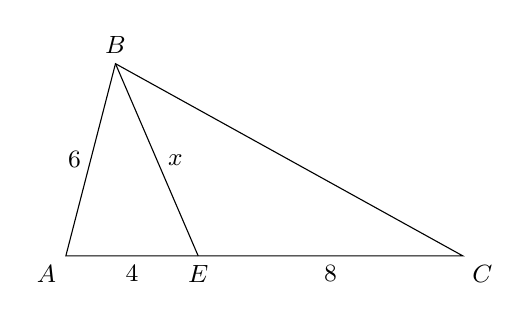
\begin{tikzpicture}[scale=0.42,font=\small]
\coordinate (A) at (0,0); \coordinate (C) at (12,0); \coordinate (B) at (1.5,5.81); \coordinate (E) at (4,0);
\draw (A)--(B)--(C)--cycle; \draw (B)--(E);
\node[below left] at (A) {$A$}; \node[above] at (B) {$B$}; \node[below right] at (C) {$C$}; \node[below] at (E) {$E$};
\node[left] at (0.75,2.9) {$6$}; \node[right] at (2.8,2.9) {$x$}; \node[below] at (2,0) {$4$}; \node[below] at (8,0) {$8$};
\end{tikzpicture}}
\Opts{$2\sqrt{10}$}{$\sqrt{10}$}{$4\sqrt{10}$}{$2\sqrt5$}}
\QQ{26}{$ABC$ uçburçakning $AB$ tomonida $D$ nuqta, $BC$ tomonida $E$ nuqta olingan. $AE$ va $CD$ kesmalar $O$ nuqtada kesişadi. Bunda $BD:AB=1:3$ va $BE:BC=1:2$. Agar $S_{ABC}=60$ bölsa, $AOC$ uçburçak yuzini toping.
\qfig{\begin{tikzpicture}[scale=0.45,font=\small]
\coordinate (A) at (0,0); \coordinate (C) at (10,0); \coordinate (B) at (7,6); \coordinate (D) at (4.667,4); \coordinate (E) at (8.5,3); \coordinate (O) at (6.8,2.4);
\fill[qfill] (A)--(O)--(C)--cycle;
\draw (A)--(B)--(C)--cycle; \draw (A)--(E); \draw (C)--(D);
\node[below left] at (A) {$A$}; \node[above] at (B) {$B$}; \node[below right] at (C) {$C$}; \node[above left] at (D) {$D$}; \node[right] at (E) {$E$}; \node[above] at (6.8,2.55) {$O$};
\end{tikzpicture}}
\Opts{$30$}{$20$}{$24$}{$28$}}
\QQ{27}{$O$ markazli aylana $ABCD$ töğri burçakli trapetsiyaga içki çizilgan. Agar $OC=2$ va $OD=4$ bölsa, trapetsiya yuzini toping.
\qfig{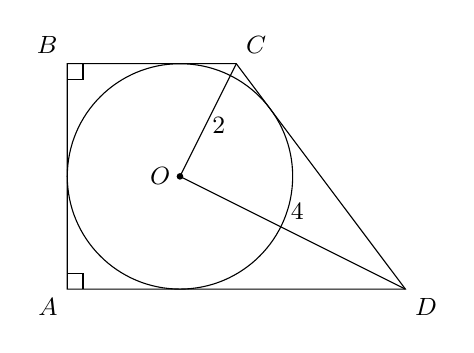
\begin{tikzpicture}[scale=0.8,font=\small]
\coordinate (A) at (0,0); \coordinate (B) at (0,3.578); \coordinate (C) at (2.683,3.578); \coordinate (D) at (5.367,0); \coordinate (O) at (1.789,1.789);
\draw (A)--(B)--(C)--(D)--cycle; \draw (O) circle (1.789); \draw (C)--(O)--(D); \fill (O) circle (1.5pt);
\draw (0,0.25)--(0.25,0.25)--(0.25,0); \draw (0,3.328)--(0.25,3.328)--(0.25,3.578);
\node[below left] at (A) {$A$}; \node[above left] at (B) {$B$}; \node[above right] at (C) {$C$}; \node[below right] at (D) {$D$}; \node[left] at (O) {$O$};
\node[right] at (2.15,2.6) {$2$}; \node[above] at (3.65,0.95) {$4$};
\end{tikzpicture}}
\Opts{$15$}{$16$}{$16\dfrac15$}{$14\dfrac25$}}
\QQ{28}{Tomoni $1$ ga teng bölgan muntazam oltiburçak tomonlarining örtalari tutaştirilib, yangi oltiburçak hosil qilindi. Hosil bölgan oltiburçak bilan ham şu jarayon çeksiz davom ettirildi. Barça oltiburçaklar yuzlarining yiğindisini toping.
\qfig{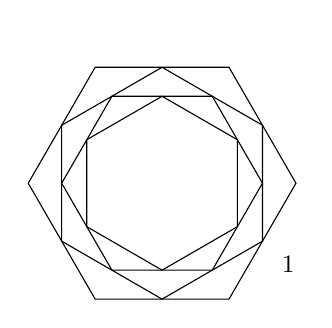
\begin{tikzpicture}[scale=1.7,font=\small]
\def\r{1}
\draw (1.0000,0.0000) -- (0.5000,0.8660) -- (-0.5000,0.8660) -- (-1.0000,0.0000) -- (-0.5000,-0.8660) -- (0.5000,-0.8660) -- cycle;
\draw (0.7500,0.4330) -- (0.0000,0.8660) -- (-0.7500,0.4330) -- (-0.7500,-0.4330) -- (-0.0000,-0.8660) -- (0.7500,-0.4330) -- cycle;
\draw (0.3750,0.6495) -- (-0.3750,0.6495) -- (-0.7500,0.0000) -- (-0.3750,-0.6495) -- (0.3750,-0.6495) -- (0.7500,-0.0000) -- cycle;
\draw (0.0000,0.6495) -- (-0.5625,0.3248) -- (-0.5625,-0.3248) -- (-0.0000,-0.6495) -- (0.5625,-0.3248) -- (0.5625,0.3248) -- cycle;
\node[above] at (90:1.02) {}; \node[below right] at (-30:0.95) {$1$};
\end{tikzpicture}}
\Opts{$10$}{$15$}{$6\sqrt3$}{$9\sqrt3$}}
\QQ{29}{$\overrightarrow{AB}(6;\,2)$ va $\overrightarrow{AC}(4;\,-12)$ bölsa, $ABC$ uçburçakka taşqi çizilgan aylana radiusini toping.
\Opts{$6\sqrt2$}{$12$}{$5\sqrt2$}{$5$}}
\QQ{30}{$\alpha$ tekislikdan taşqarida joylaşgan $A$ nuqtadan uşbu tekislikka $AB$ va $AC$ oğmalar hamda $AH$ perpendikulyar tuşirilgan. Bu yerda $H$ — perpendikulyarning asosi bölib, $B$, $C$ va $H$ nuqtalar $\alpha$ tekislikda yotadi. Agar $AH=4$, $\angle ABH=45^\circ$, $\angle ACH=60^\circ$, $\angle BHC=60^\circ$ bölsa, $AHBC$ piramidaning hajmini toping.
\Opts{$6\dfrac23$}{$5\dfrac23$}{$5\dfrac13$}{$6\dfrac13$}}
\QQ{31}{$A=\{1;\,2;\,3;\,4;\,5;\,6\}$ töplamning $3$ yoki $5$ elementlaridan kamida bittasini öz içiga olgan qism töplamlari neçta?
\Opts{$56$}{$48$}{$32$}{$16$}}
\QQ{32}{$1000$ gaça bölgan natural sonlar içida $11$ ga qoldiqsiz bölinadigan, $2$ ga ham, $3$ ga ham qoldiqsiz bölinmaydigan sonlar neçta?
\Opts{$90$}{$75$}{$45$}{$30$}}
\QQ{33}{\Moslash{Konus, silindr va şar hajmlari özaro teng. Silindrning öq kesimi kvadratdan, konusning öq kesimi esa teng tomonli uçburçakdan iborat.
\par\centering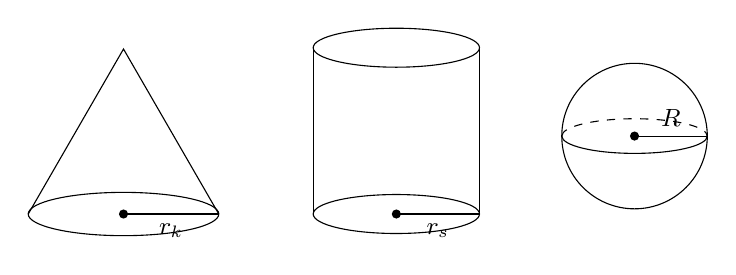
\begin{tikzpicture}[scale=0.55,font=\small]
\draw (0,0) ellipse (2.2 and 0.5); \draw (-2.2,0)--(0,3.81)--(2.2,0); \draw (0,0)--(2.2,0); \fill (0,0) circle (3pt); \node[below] at (1.1,0) {$r_k$};
\begin{scope}[xshift=6.3cm]
\draw (0,0) ellipse (1.92 and 0.45); \draw (0,3.84) ellipse (1.92 and 0.45); \draw (-1.92,0)--(-1.92,3.84); \draw (1.92,0)--(1.92,3.84);
\draw (0,0)--(1.92,0); \fill (0,0) circle (3pt); \node[below] at (0.96,0) {$r_s$};
\end{scope}
\begin{scope}[xshift=11.8cm,yshift=1.8cm]
\draw (0,0) circle (1.68); \draw[dashed] (-1.68,0) arc (180:0:1.68 and 0.4); \draw (-1.68,0) arc (180:360:1.68 and 0.4);
\draw (0,0)--(1.68,0); \fill (0,0) circle (3pt); \node[above] at (0.84,0) {$R$};
\end{scope}
\end{tikzpicture}}{A) $\dfrac{\sqrt[6]{12}}2$\par B) $\dfrac{\sqrt[6]3}{\sqrt[3]6}$\par C) $\dfrac{\sqrt[3]{18}}2$\par D) $\dfrac{\sqrt[3]{12}}6$\par E) $\dfrac{\sqrt[3]{18}}3$\par F) $\dfrac{\sqrt[3]6}2$}{Silindr asosi radiusining konus asosi radiusiga nisbatini toping.}{Şar radiusining konus asosi radiusiga nisbatini toping.}{Silindr asosi radiusining şar radiusiga nisbatini toping.}}
\QQ{36}{Tenglamani yeçing:
\[2\left(x^2+x+1\right)^2-13\left(x^3-1\right)=7(x-1)^2\]
\AB{Tenglama neçta haqiqiy ildizga ega?}{Tenglamaning haqiqiy ildizlari köpaytmasini toping.}}
\QQ{37}{Tenglamani yeçing:
\[(\sin x+\cos x)^4+(\sin x-\cos x)^4+\sin4x=3\]
\AB{Tenglamaning eng kiçik musbat yeçimini toping.}{Tenglama $[-\pi;\,2\pi]$ oraliqda neçta yeçimga ega?}}
\QQ{38}{$f(x)$ funksiya barça $x\ne0$, $x\ne1$ larda quyidagi tenglikni qanoatlantiradi:
\[2f(x)+f(1-x)=\frac{3x^2+x+4}{x(1-x)}\]
$f^{-1}(x)$ — $f(x)$ ga teskari funksiya.
\AB{$f(2)$ ni toping.}{$f^{-1}(-2)$ ni toping.}}
\QQ{39}{$f(x)=2\sqrt x$ funksiya berilgan.
\qfig{\begin{tikzpicture}[scale=0.55,font=\small]
\draw[-{Stealth[length=4pt]}] (-4,0)--(9,0) node[right] {$x$}; \draw[-{Stealth[length=4pt]}] (0,-1)--(0,7.2) node[left] {$y$};
\draw[thick,domain=0:8.5,samples=80] plot (\x,{2*sqrt(\x)}) node[right] {$y=2\sqrt x$};
\draw[domain=-3.5:7,samples=2] plot (\x,{\x/2+3}) node[above left] {$y=\frac x2+3$};
\node[below left] at (0,0) {$O$};
\end{tikzpicture}}
\AB{$f(x)$ funksiya grafigiga ötkazilgan urinma $Ox$ öqi bilan $30^\circ$ li burçak hosil qiladi. Urinmaning $Ox$ öqi bilan kesişiş nuqtasidan $y=2\sqrt x$ funksiya grafigigaça bölgan eng qisqa masofani toping.}{$y=2\sqrt x$ funksiya grafigidan $y=\dfrac x2+3$ töğri çiziqqaça bölgan eng qisqa masofani toping.}}
\QQ{40}{$f(x)=x^3+ax^2+bx+c$ funksiya grafigi $Ox$ öqini $(-1;\,0)$ nuqtada kesib ötadi va $(2;\,0)$ nuqtada urinadi.
\qfig{\begin{tikzpicture}[xscale=0.9,yscale=0.55,font=\small]
\fill[qfill] (-1,0)--plot[domain=-1:2,samples=60] (\x,{(\x+1)*(\x-2)*(\x-2)})--cycle;
\draw[-{Stealth[length=4pt]}] (-2.2,0)--(3.4,0) node[right] {$x$}; \draw[-{Stealth[length=4pt]}] (0,-2)--(0,6) node[left] {$y$};
\draw[thick,domain=-1.4:2.9,samples=80] plot (\x,{(\x+1)*(\x-2)*(\x-2)});
\node[below left] at (-1,0) {$-1$}; \node[below] at (2,0) {$2$}; \node[below left] at (0,0) {$O$};
\end{tikzpicture}}
\AB{$a+b+c$ ni toping.}{Funksiya grafigi va $Ox$ öqi bilan çegaralangan soha yuzini toping.}}
\QQ{41}{Tomonlari $2$, $4$ va $6$ ga teng bölgan $ABCD$, $DEFN$ va $NMKL$ kvadratlar rasmda körsatilgandek joylaşgan. $AK$ kesma $DE$ va $NM$ tomonlarni mos ravişda $R$ va $T$ nuqtalarda kesib ötadi.
\qfig{\begin{tikzpicture}[scale=0.5,font=\small]
\fill[qfill] (2,0)--(2,1)--(6,3)--(6,0)--cycle;
\draw (0,0) rectangle (2,2); \draw (2,0) rectangle (6,4); \draw (6,0) rectangle (12,6); \draw (0,0)--(12,6);
\node[below left] at (0,0) {$A$}; \node[above left] at (0,2) {$B$}; \node[above] at (2,2) {$C$}; \node[below] at (2,0) {$D$};
\node[above left] at (2,4) {$E$}; \node[above] at (6,4.05) {$F$}; \node[below] at (6,0) {$N$};
\node[above left] at (6,6) {$M$}; \node[above right] at (12,6) {$K$}; \node[below right] at (12,0) {$L$};
\node[right] at (2,1.2) {$R$}; \node[below right] at (6,3) {$T$};
\end{tikzpicture}}
\AB{Böyalgan $DRTN$ soha yuzini toping.}{$|TK|$ ni toping.}}
\QQ{42}{Katetlari $AC=3$ va $AB=4$ bölgan $ABC$ töğri burçakli uçburçakning $BC$ va $AC$ tomonlariga taşqi tomondan $BCFE$ va $ACML$ kvadratlar qurilgan. $O_1$ va $O_2$ — mos ravişda $ACML$ va $BCFE$ kvadratlarning markazlari.
\qfig{\begin{tikzpicture}[scale=0.7,font=\small]
\coordinate (A) at (0,0); \coordinate (B) at (0,4); \coordinate (C) at (3,0); \coordinate (L) at (0,-3); \coordinate (M) at (3,-3);
\coordinate (F) at (7,3); \coordinate (E) at (4,7); \coordinate (O1) at (1.5,-1.5); \coordinate (O2) at (3.5,3.5);
\fill[qfill] (A)--(O1)--(O2)--cycle;
\draw (A)--(B)--(C)--cycle; \draw (A)--(C)--(M)--(L)--cycle; \draw (B)--(C)--(F)--(E)--cycle; \draw (A)--(O1)--(O2)--cycle; \draw (M)--(F);
\draw (0,0.3)--(0.3,0.3)--(0.3,0);
\fill (O1) circle (2pt); \fill (O2) circle (2pt);
\node[left] at (A) {$A$}; \node[above left] at (B) {$B$}; \node[right] at (3.05,0.1) {$C$}; \node[below left] at (L) {$L$}; \node[below right] at (M) {$M$};
\node[right] at (F) {$F$}; \node[above] at (E) {$E$}; \node[below] at (O1) {$O_1$}; \node[above] at (O2) {$O_2$};
\end{tikzpicture}}
\AB{$|MF|$ ni toping.}{$AO_1O_2$ uçburçak yuzini toping.}}
\QQ{43}{$ABCD$ trapetsiya ($BC\parallel AD$) aylanaga içki çizilgan. $BC=3$, $AD=13$. Aylanada $E$ nuqta ($E\ne D$) şunday olinganki, $BE=BD=10$.
\qfig{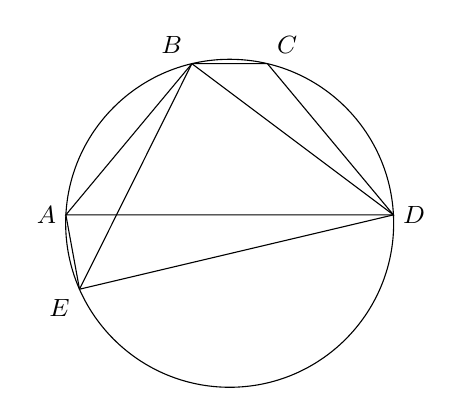
\begin{tikzpicture}[scale=0.32,font=\small]
\coordinate (A) at (-6.5,0); \coordinate (D) at (6.5,0); \coordinate (B) at (-1.5,6); \coordinate (C) at (1.5,6); \coordinate (E) at (-5.959,-2.95); \coordinate (O) at (0,-0.333);
\draw (O) circle (6.5085); \draw (A)--(B)--(C)--(D)--cycle; \draw (B)--(D); \draw (B)--(E); \draw (A)--(E)--(D);
\node[left] at (A) {$A$}; \node[above left] at (B) {$B$}; \node[above right] at (C) {$C$}; \node[right] at (D) {$D$}; \node[below left] at (E) {$E$};
\end{tikzpicture}}
\AB{$AE$ ni toping.}{$ABCDE$ beşburçak yuzini toping.}}
\QQ{44}{Jism yarim şar, silindr va konusdan taşkil topgan. Yarim şar, silindr va konus asoslarining radiusi $3$ cm, konusning yasovçisi $5$ cm, jismning umumiy uzunligi $15$ cm.
\qfig{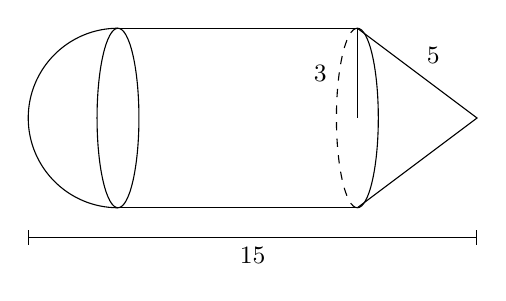
\begin{tikzpicture}[scale=0.38,font=\small]
\draw (3,3) arc (90:270:3); \draw (3,3)--(11,3); \draw (3,-3)--(11,-3); \draw (11,3)--(15,0)--(11,-3);
\draw (3,0) ellipse (0.7 and 3); \draw (11,-3) arc (-90:90:0.7 and 3); \draw[dashed] (11,3) arc (90:270:0.7 and 3);
\draw (11,0)--(11,3); \node[left] at (10.3,1.5) {$3$}; \node[above right] at (13,1.5) {$5$};
\draw[|-|] (0,-4)--(15,-4); \node[below] at (7.5,-4) {$15$};
\end{tikzpicture}}
\AB{Jismning töla sirtini toping (cm$^2$).}{Jismning hajmini toping (cm$^3$).}}
\QQ{45}{Quyida osma köprik parabola şaklida tasvirlangan. Köprikning eng katta ustunlari orasidagi masofa $300$ m, qolgan ustunlar orasidagi masofalar $15$ m dan va katta ustun balandligi $67$ m ga teng. Köprik markaziga koordinata boşi, yaʼni $O(0;\,0)$ nuqta joylaştirilgan.
\qfig{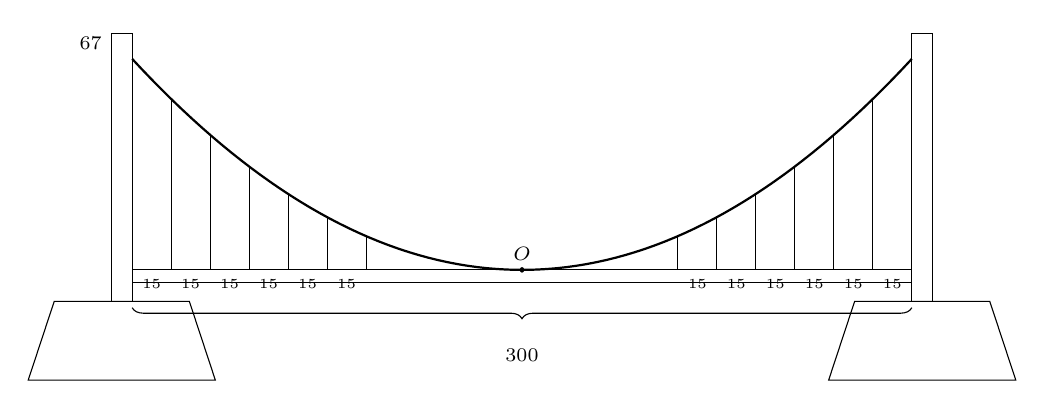
\begin{tikzpicture}[xscale=0.033,yscale=0.04,font=\scriptsize]
\draw (-158,-10) rectangle (-150,75); \draw (150,-10) rectangle (158,75);
\draw[thick,domain=-150:150,samples=80] plot (\x,{67*(\x/150)*(\x/150)});
\draw (-150,0)--(150,0); \draw (-150,-4)--(150,-4);
\foreach \x in {-135,-120,...,-60,60,75,...,135} \draw (\x,0)--(\x,{67*(\x/150)*(\x/150)});
\fill (0,0) circle (25pt); \node[above] at (0,0) {$O$};
\foreach \x in {-150,-135,...,-75,60,75,...,135} \node[below] at (\x+7.5,0) {\tiny 15};
\draw[decorate,decoration={brace,mirror,amplitude=4pt}] (-150,-12)--(150,-12); \node[below] at (0,-22) {$300$};
\draw (-190,-35)--(-180,-10)--(-128,-10)--(-118,-35)--cycle; \draw (118,-35)--(128,-10)--(180,-10)--(190,-35)--cycle;
\node[left] at (-158,72) {$67$};
\end{tikzpicture}}
\AB{Parabola tenglamasini tuzing.}{$12$ ta kiçik ustunlar uzunliklari yiğindisini toping.}}
\Javoblar{C B C A C A B A C B A A B D A A D A A B A D C A A C D C C C B D B A E}{\OK{36}{$4$}{$4$}\OK{37}{$\dfrac\pi{16}$}{$12$}\OK{38}{$-5$}{$5$}\OK{39}{$3$}{$\dfrac{2\sqrt5}5$}\OK{40}{$1$}{$\dfrac{27}4$}\OK{41}{$8$}{$3\sqrt5$}\OK{42}{$2\sqrt{13}$}{$\dfrac{21}4$}\OK{43}{$3$}{$\dfrac{4098}{61}$}\OK{44}{$81\pi$}{$102\pi$}\OK{45}{$y=\dfrac{67}{22500}x^2$}{$363{,}14$}}
